\chapter{EXISTING DESIGNS AND PRODUCTS}\label{chap2}
\thispagestyle{empty}

%In this chapter you have to provide the results of your preliminary and detail searches related to the topic conducted to find out the existing products, designs and ideas. Refer to the all available sources that you searched and obtained results related to it. It can go up to many designs/products/ideas.

\section{Conventional Vending Machine}
A vending machine is an automated machine that provides items such as snacks, beverages, and other items to consumers after inserting money, a credit card or a specially designed card into the machine. They are a huge convenience for the users as they are easy to operate and the products are received quickly.

\begin{figure}[h]
	\centering
	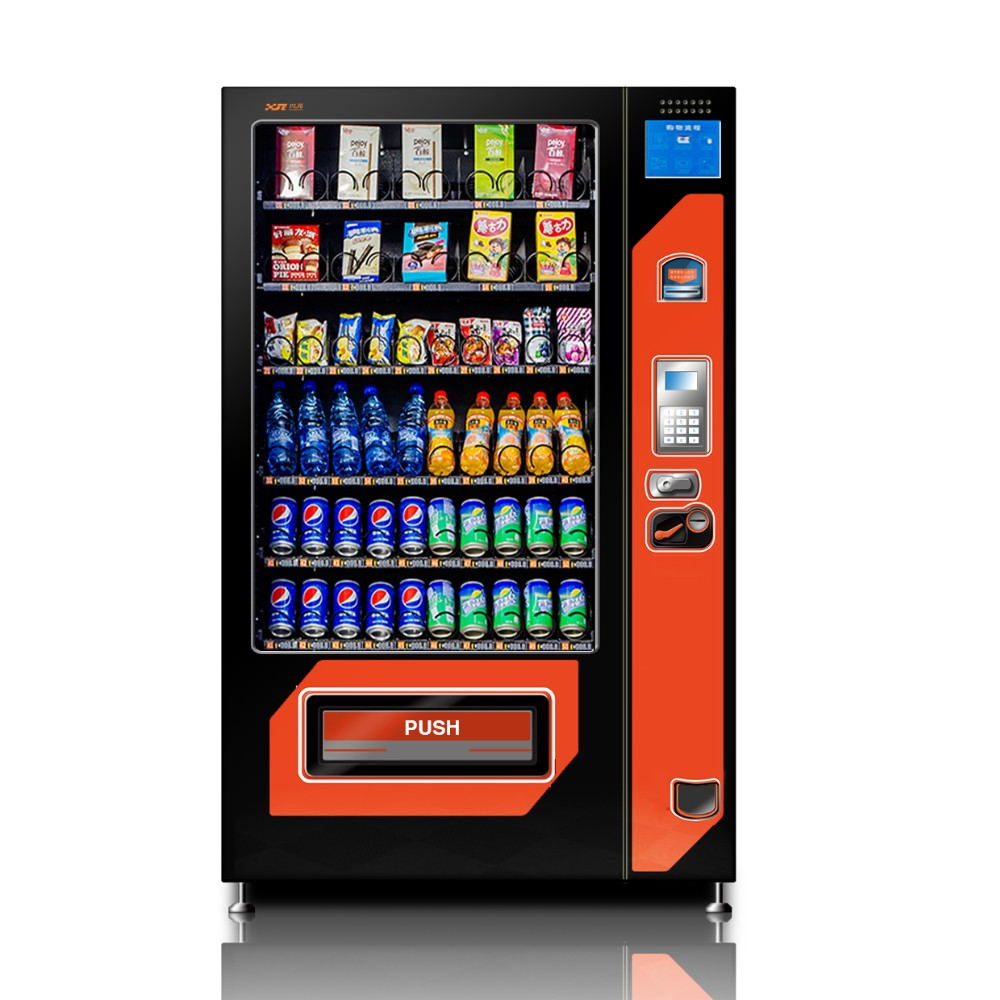
\includegraphics[width=0.85\linewidth]{./picture-files/vending_machine.jpg}
	\caption{A vending machine}
	\label{fig:VenMach}
\end{figure}

But the proposed Paper Pen Vending Machine does not accept any coin or credit card payments like conventional vending machines. Instead, it accepts three waste plastic pens and provides a paper pen in return. Accepting waste plastic pens promotes the necessity for proper disposal of them and also encourages the user to use the machine as it does require any monetary element and rewards the user with, practically, a free paper pen.

\section{Tensorflow and Image Classification}\label{tf_sec}

TensorFlow is an end-to-end open source platform for machine learning. It has a comprehensive, flexible ecosystem of tools, libraries and community resources that lets researchers push the state-of-the-art in ML and developers easily build and deploy ML powered applications.\cite{TensorFlow}

An article by IBM developers ``Image recognition with TensorFlow and Keras" \cite{ibm}, demonstrates the basic image classification algorithm. The code teaches the computer to distinguish between chihuahua and muffin which look similar. This code was utilized to do the same function with pens. 

\section{Terracycle Zero Waste Box\texttrademark }

\subsection{TerraCycle}TerraCycle is a private U.S. recycling business headquartered in Trenton, New Jersey. It primarily runs a volunteer-based curbside collection program to collect non-recyclable pre-consumer and post-consumer waste, and then partners with corporate donors or municipalities to turn it into raw material to be used in new products. The company licenses its name to manufacturers of roughly 200 products made using its raw material. TerraCycle also manages Loop, a consumer products shopping service with reusable packaging.\cite{tcycle}

\subsection{The program and collected wastes}
TerraCycle has created the program named Zero Waste Box\texttrademark   as a solution for pens, pencils, and markers as waste to the environment. A box is utilized to collect waste writing instruments and recycle this collected waste. The collected wastes consist of pens and pen caps, mechanical and wooden pencils, markers and marker caps, permanent markers, and permanent marker caps.

\subsection{Processing of the waste}
Once collected, the waste writing instruments are separated by material composition. The separated items are then cleaned, shredded, and made into new recycled products.

\section{Summary}
This chapter has discussed how the PPVM is different from conventional vending machines, what utilities were used for the software part, and how the collected pens can be recycled. From these discussions, it is possible to see the practicality of the PPVM. 
